\subsection{Training}
    
    For training, we use a pretrained version of MobileNetV2 \cite{mobilenetv2} on ImageNet \cite{imagenet}, and for the optimizer we use Adam. We use a cosine annealing scheduler for the learning rate, described in \cite{cosine_scheduler}, which follows the following formula:
    
    \begin{equation}
        LR_{epoch} = \eta_{min} + \frac{1}{2} (\eta_{max} - \eta_{min}) \cdot (1 + cos(\frac{epoch}{T} \cdot \pi))
        \label{cosine_formula}
    \end{equation}
    
    The main idea is that the learning rate will follow a cosine wave between $\eta_{min}$ and $\eta_{max}$. The epoch represents the current epoch, and $T$ represents the restart epoch, meaning that every $T$ epochs the monotony is changed, and the learning rate will reach either $\eta_{min}$ or $\eta_{max}$. %We can better see the phenomenon in Fig. \ref{scheduler}, where various schedules for the learning rate are plotted over a total of 50 epochs. We can see that when $T$ is equal to the total number of epochs, the learning rate decreases monotonously from the maximum to the minimum. If $T$ is larger than the number of epochs, then the learning rate doesn't even reach the minimum, and if the learning rate is smaller than the number of epochs, the cosine wave can be seen, and every $T$ epochs, the slope changes.
    
    %\begin{figure}[t]
    %    \centering
    %    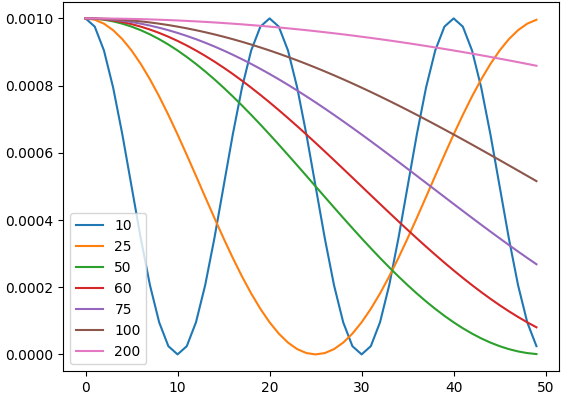
\includegraphics[scale=0.4]{images/scheduler.png}
    %    \caption{Cosine annealing scheduler}
    %    \label{scheduler}
    %\end{figure}
    
    
    
    We train the model for 50 epochs on a GPU using early stop with the patience of 5 epochs and a delta of $1e^{-4}$. This means that if the model does not improve after some epochs, by the given delta, the training stops because we don't want to overtrain, in order to both save time and reduce overfitting also.
    
    At the beginning of the epoch, the learning rate is set, following the cosine annealing formula, and at the end, the images are shuffled in order for the network to see the images in a different order, each epoch. Also, during training, before any processing, random photometric data augmentation is used, followed by cutout and mosaic as explained in a previous section.
    
    During a normal training session, the weights of the pretrained model are frozen, meaning that they do not update. We do this in order to not break the knowledge stored in the weights. But, during a fine tuning session, which occurs after a normal training session, we set a very small learning rate and unfreeze the pretrained model. By doing this, the previously frozen weights are updated to better fit our dataset. Usually, a fine tuning epoch takes much longer, because the pretrained model has the largest share in parameters of the total number of parameters.

     In Fig. \ref{model_v42_loss} we present the evolution of the loss during training for our best model. Ideally, the validation loss is always around the training loss. This is a sign that the model does not overfit.
     
     \begin{figure}[b]
        \centering
        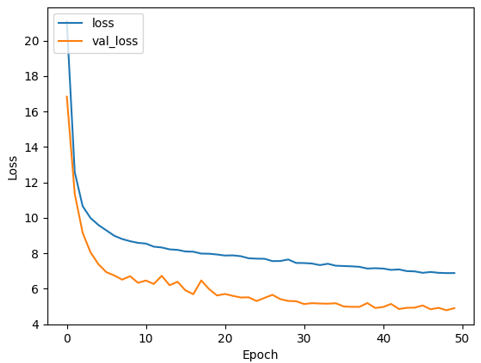
\includegraphics[scale=0.25]{images/model_v42_train.png}
        \caption{Training (blue) and validation (orange) loss for our best model}
        \label{model_v42_loss}
    \end{figure}